\documentclass[12pt,letterpaper]{article}


%\usepackage{amsthm}
\usepackage{multirow}
\usepackage{graphicx}
%\usepackage{epsfig}
%\usepackage{subfigure}
\usepackage{amsmath}
\usepackage{indentfirst}
\usepackage{amssymb}
\usepackage{cases}
\usepackage{ dsfont }
\usepackage[figuresright]{rotating}
\usepackage{float}
%\usepackage{subfigure}
\usepackage{caption}
 \usepackage{subcaption}
\usepackage[superscript,biblabel]{cite}

\DeclareMathOperator*{\argmax}{arg\,max}

\usepackage{setspace}
\onehalfspacing


\newtheorem{theorem}{Theorem}
\newtheorem{lemma}{Lemma}
\newtheorem{alg}{Algorithm}
\newtheorem{definition}{Definition}
%{\noindent{\bfseries Proof}}
\newcommand{\Proof}{\noindent{\bfseries Proof}}
%\newcommand{\be}{\begin{equation}}
%\newcommand{\ee}{\end{equation}}
\newtheorem{corollary}{Corollary}
\newtheorem{proposition}{Proposition}
\newtheorem{conjecture}{Conjecture}


\newcommand{\MyTabs}{ \hspace*{15.mm} \= ... \kill }


\usepackage[top=1in, left=1in, right=1in, bottom=1in]{geometry}

\newcommand{\tinyth}{\mbox{{\tiny{th}}}}
\newcommand{\tinyst}{\mbox{{\tiny{st}}}}

\usepackage{sectsty}

\sectionfont{\fontsize{12}{15}\selectfont}

\usepackage{abstract}
\renewcommand{\abstractname}{}    % clear the title
\renewcommand{\absnamepos}{empty} % originally center

\begin{document}
\renewcommand{\refname}{REFERENCES}

\title{XXX}

\author {xxx}%\Large 

\date{}

\maketitle

\begin{abstract}
\noindent\looseness-1
xxx
\end{abstract}

%\begin{keywords}
%Virtual Age, Remote Transmission, Finite Horizon\\
%\end{keywords}
%\centerline{\textsc{acronyms}}
%\begin{tabbing} \MyTabs
%PM\>preventive maintenance \\
%\end{tabbing}
%\centerline{\textsc{notation}}
%\begin{tabbing} \MyTabs
%$L$\> initial system lifetime \\
%\end{tabbing}


%\section*{Introduction}\label{sec:Intro}
%\baselineskip 20pt plus .3pt minus .1pt
\looseness - 1




\section*{Introduction}

\looseness - 1
Sleep is a natural part of every person's life. One-third of every individual's live is spent in the sleeping state. Many restorative functions of body including physical recreation and immune functions as well as mental restoration, memory consolidation, mood and behavior are dependent on a healthy sleep. Deprivation of sleep can lead to rising risk of serious health problems such as heart diseases, obesity, diabetes and weakness of immunity system. 
Sleep is not a homogeneous process. It has an internal cyclical structure. Rechtschaffen and Kales (R-K) (1968) introduce sleep stages based on visual observations of the patterns and signals of electroencephalography (EEG), Electrooculography (EOG), and Electromyography (EMG). This standard method of sleep evaluation is called polysomnography (PSG). Based on R-K sleeping criteria, sleep stages are defined as: awake, rapid eye movement (REM) and non-rapid eye movement (NREM) which including stages 1, 2, 3 and 4. Sleep stages 3 and 4 are often combined together and considered as one sleep stage. Due to the complicated system of PSG recording which is costly, time consuming and uncomfortable for the patient, automatic sleep scoring system could be very helpful. Several automatic sleep staging methods have been published in the literature. For convenience of comparing these method, we introduce the literature in five categories of dataset, channels, features, algorithms and accuracy.
 
\section*{Literature Review}
\looseness - 1
\subsection*{ Dataset:}

\subsubsection*{Physionet online dataset}

The EEG dataset is publicly available online at PhysioBank [8]. The polysmnographic (PSG) sleep recordings included signals from EEG ( Fpz-Cz and Pz-Oz channels), horizontal EOG, submental chin EMG and an event marker. Well-trained technicians scored manually hypnograms based on the 1968 Rechtschaffen and Kales manual [9].
There are two subsets of data. In the first set, 20 healthy subjects were selected in order to study the effects of age on sleep. Two EEG datasets (about 20 hours) were recorded during two subsequent day-night periods for each subject at their home. In the second dataset, 22 subjects that had difficulty in falling sleep were selected from a study of Temazepam effects on sleep. The PSGs (about 9 hours) were recorded in the hospital during two nights.
\subsubsection*{Dataset used by previous studies}
Oropesa et al. (1999) use 30-second epochs from two EEG recordings as a dataset. Zoubek et al. (2007) use 20-second epochs of 47 night sleep recordings of healthy adults. Doroshenkov et al. (2007) use the recordings of two EEG channels (Fpz-Cz and Pz-Oz) of eight subjects (without using any medications) from physionet online dataset. Sinha (2008) uses five subjects from normal human and without any type of sleep stimulating agent. Ebrahimi et al. (2008) use seven EEG recordings from physionet online dataset. Gunes et al. (2009) use three night sleep recording. Jo et el. (2010) use four healthy subjects which do not use any medications and have no sleep disorders. Tagluk et al. (2009) obtain the dataset from seven hours sleep recording of 21 subjects. Fraiwan et al. (2011) use the recordings of an entire night of sleep (6–8 h) of sixteen subjects. Ozsen et al. (2012) use five sleep recordings. Koley and Dey (2012) use recordings of 28 subjects (having sleep apnea) during one night sleep. Liang et al. (2012) use the recordings of 20 healthy subjects. Hsu et al. (2013) use the recordings of eight subjects during 24 hour of daily life (physionet online dataset). 
\subsection*{ Channels:} 

Most of previous works use multiple channels including EEG channels, EOG and EMG channels. Oropesa et al.\ use 30-second epochs of two separate EEG channels. Zoubek et al.\ use 20-second epochs of four EEG channels (C3-A2, P3-A2, C4-A1, and P4-A1) from 47 night sleep recordings of healthy adults. By including the features extracted from EOG and EMG channels, Zoubek et al.\ improve the accuracy of the same classification algorithm. Doroshenkov et al.\ use the recordings of two EEG channels (Fpz-Cz and Pz-Oz) of eight subjects (without using any medications) from physionet online dataset. Tagluk et al.\ obtain the dataset from seven hours sleep recording of 21 subjects which including an EEG channel (C3-A2), EMG and EOG. Fraiwan et al.\ use a single EEG channel (C3-A1) for an entire night of sleep (6–8 h) of sixteen subjects. Ozsen et al. (2012) use five sleep recordings of EEG, EMG and EOG. Koley and Dey\ use single channel EEG (C4-A1) recordings of 28 subjects (having sleep apnea) during one night sleep. Liang et al. (2012) use the recordings of 20 healthy subjects of single EEG channel (C3-A2). Hsu et al.\ use single EEG channel (Fpz-Cz) of eight subjects during 24 hour of daily life (physionet online dataset). However, there are a few works which consider only one EEG channel for prediction. Ebrahimi et al.\ use 30-second epochs of seven EEG recordings from physionet online dataset of Pz-Oz channel. Jo et el.\ use 30-second long epochs of a single channel EEG signal (C3-A2) use a single EEG channel (C3-A1) for an entire night of sleep (6-8 h) of sixteen subjects.
\subsection*{ Features:}

Oropesa et al.\ use discrete wavelet transform (DWT) to extract energy from seven EEG subbands as features and use them in their classification algorithm along with an additional six more features based on total energy and the relative energy of subbands. Zoubek et al.\ apply both DWT and fast fourier transform (FFT) to extract features. They use relative wavelet energy of five EEG subbands as features. Doroshenkov et al.\ use FFT to extract four features of subbands. Ebrahimi et al.\ use energy, total energy, ratio of different energy values of six subbands accordingly as well as mean of the absolute values of the coefficients and standard deviation of the coefficients in each subband. Gunes et al.\ extract 258 features by applying Welch method for EEG and chin EMG signals. They use statistical measures including minimum value, maximum value, standard deviation, and mean value belonging to each feature in sleep stage dataset in order to decrease to 8 features for EEG and chin EMG signals. Fraiwan et al.\ use three different methods of time-frequency analysis to extract the features: Choi–Williams distribution (CWD), Continuous wavelet transform (CWT) and Hilbert–Huang Transform (HHT). Fraiwan et al.\ extract seven features by computing Renyi’s entropy of subbands. Ozsen et al.\ extract 57 features from EEG, EMG, left and right EOG signals. These features are mainly statistical features of signal (mean, standard deviation, skewness, kurthosis,etc) as well as power features of subbands. They use FFT to extract power features of subbands. Koley and Dey\ extract 39 features including time domain, frequency domain and non-linear analysis (21 features finally selected. Liang et al.\ use the features of multiscale entropy (MSE) and auto regressive (AR). Hsu et al.\ apply FFT to extract six (alpha, beta, theta, delta, spindle, and sawtooth) energy features of subbands.

\subsection*{ Algorithms:}

Oropesa et al.\ use artificial neural network (ANN) algorithm. Zoubek et al.\ apply three different classifiers including two bayes rule-based classifiers (parametric and non-parametric ones) as well as multi-layer perceptron (MLP). Doroshenkov et al.\ use the classification approach based on Hidden Markov Model (HMM). Sinha\ and Ebrahimi et al.\ apply ANN as a classifier. Gunes et al. (2009) use C4.5 decision tree to classify sleep stages. Jo et el.\ design the fuzzy classifier based on the genetic algorithm (GA). Tagluk et al.\ use multi-layer NN classifier. Fraiwan et al.\ apply Random forest (RF) as a classifier. Ozsen et al.\ use ANN to classify sleep stages. Koley and Dey\ use support vector machine (SVM) as a classifier. Hsu et al.\ apply NN to classify sleep stages. 
\subsection*{ Accuracy:}

Oropesa et al.\ obtain the total accuracy of $77.6\%$ which including $65\%, 74\%, 90.5\%$ and $75\%$ for REM, awake, stage 1 (S1) and stage 2 (S2), respectively. Zoubek et al.\ obtain an accuracy of $71\%$. By including the features extracted from EOG and EMG channels, Zoubek et al.\ improve the accuracy of the same classification algorithm to around $80\%$. Doroshenkov et al.\ achieve the accuracy of$ 51.04\%, 4.84\%, 68.62\%, 64.13\%, 91.54\% $and $86.32\%$ for awake, S1, S2, S3, S4 and REM, respectively. Sinha\ classifies three stages of sleep: awake (AWA), rapid eye movement (REM) and sleep spindles (SS) and obtain accuracy of $95.52\%, 93.38\%$ and $95.52\% $, respectively. Sinha achieves the total accuracy of $95.35\%$.  Ebrahimi et al.\ achieve the accuracy rate of $98.5\%, 91.4\%, 87.5\%, 94.6\%$ and $93\%$ for awake, S1+REM, S2, slow wave stage (SWS) and total accuracy, respectively. Gunes et al.\ achieve the success rate of $28.3\%, 0.0\%, 68.6\%, 10\%, 40.5\%$ and $92.5\% $for awake, S1, S2, S3, REM and non-sleep (movement time). Jo et el.\ obtain the accuracy rate of $86.4\%, 83.9\%, 84.3\%, 85.5\%$ and $84.6\%$ for awake, shallow sleep (SS), deep sleep (DS), REM and total accuracy. Tagluk et al.\ obtain the accuracy of $72.6\%, 73.3\%, 78\%, 72.3\%, 77.3\%$ and $74.7\%$ for S1, S2, S3, S4, REM and total accuracy. Fraiwan et al.\ obtain the accuracy rate of $83\%$, $78\%$ and $75\%$ for CWT, CWD and HHT , respectively. Ozsen et al.\ obtain the total accuracy rate of $90.93\%$. Koley and Dey (2012) achieve the accuracy rate of $91.1\%$. Liang et al.\ obtain the accuracy of $86.28\%, 28.45\%, 88.09\%, 86.68\%, 97.63\%$ and $88.11\%$ for S1, S2, SWS, REM and total accuracy. Hsu et al.\ achieve the accuracy rate of $70.8\%, 89.5\%, 36.7\%, 97.3\%, 89.7\%$ and $87.2\%$ for awake, REM, S1, S2, SWS and the total accuracy.\\

 
The purpose of this present study is to develop an automatic sleep staging system based on single-channel EEG for patient convenience. In this study, EEG signal is acquired from Fpz-Cz channel of physionet online dataset and divided to 10-second epochs. Seven features are extracted from time-frequency domain of signal. The number of features used in this study is smaller than that of previous works. The novel method of structuring of features is proposed in this paper which considers the previous layers of features simultaneously. By using this method of structuring dataset and RF as a classifier, we succeed to obtain the higher classification accuracy for total accuracy as well as accuracy of each sleep stages (specially stage 1). 





\section*{Wavelet Transform}

Wavelet transform (WT) is a powerful technique in signal processing for solving various real-life problems. This method analyzes non-stationary signals which frequency responses varies in time in both time and frequency [1,2]. Wavelet is a small wave which its energy is concentrated in time to analyze EEG signal as a non-stationary signal.

Wavelet analysis measures the frequency similarity between the signal and the original wavelet(mother wavelet).
In WT, computations are done for different frequency components (scale) by shifting the time window until the wavelet reaches at the end of the signal[3].WT has a precise time resolution at high frequencies and good frequency resolution at low frequencies. With this feature, WT helps the analysis of non-stationary signals[4].


The continuous wavelet transform (CWT) of a signal, x(t), is defined as follows,  \\
$CWT(a,b)=\int_{-\infty}^{\infty} x(t)\frac{1}{\sqrt{|a|}}\psi(\frac{(t-b)}{a})dt$ \\

The coefficients of CWT are computed within this formula by the integral of the original signal which is multiplied by a mother wavelet w. The scaling parameter(a) is related to frequency. High scales correspond to low frequencies which give information of the entire signal whereas low scales (high frequencies) give detailed information in the signal. The parameter b corresponds to the location of time window which is shifted over the length of the signal. In fact, CWT measures the similarity of the frequency in the original signal and the mother wavelet.
The CWT has a weak point for calculating coefficients at each scale. Because it requires expensive computational task as the matter of redundancy.   
The Discrete Wavelet Transform (DWT)solves this problem by operating filtering tasks.In this procedure, the signal is passed through a half band low pass filter which results removing some samples from signal. Therefore, the scales and time window shifts are chosen based on powers of two (dyadic). The DWT is defined as,\\  

$DWT(j,k)=\frac{1}{\sqrt{|2^j|}}\int_{-\infty}^{\infty}x(t)\psi(\frac{(t-2^jk)}{2^j})dt$\\

where a and b in the CWT are replaced by $2^j$ and $2^jk$, respectively.
At every level of the DWT, the signal is  passed through a low pass (LP) and high pass (HP) filters which results in half number of samples and half the frequency. The outputs of LP and HP at each level i are called approximation (Ai) and detail (Di) coefficients , respectively. Fig. 1 shows the wavelet decomposition of a signal through 3 levels of filtering. In this figure, the coefficients A1, D1, A2, D2, A3 and D3 are the DWT coefficients which includes the frequency content of the original signal within the
bands ${0-\frac{fs}{2}},{\frac{fs}{2}-fs}, {0-\frac{fs}{4}}, {\frac{fs}{4}-\frac{fs}{2}},{ 0-\frac{fs}{8}}$ and ${\frac{fs}{8}-\frac{fs}{4}}$, respectively where fs is the sampling rate( frequency) of the original signal x[n].\\
\begin{figure}

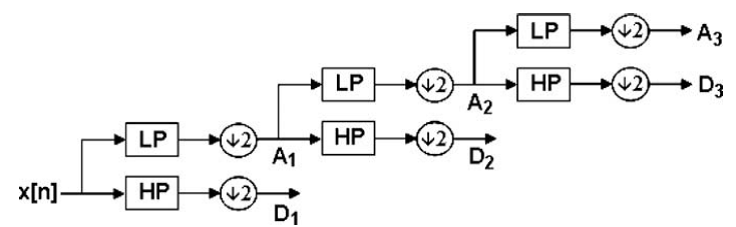
\includegraphics[width=1\textwidth]{graph.png}

\caption{Sub-band decomposition of DWT implementation}
\end{figure}
In the figure, the discrete x(n) signal crosses has the sampling rate of (100Hz) which passes iteratively through HP to generate detail coefficients (Di[n]) and crosses through LP to obtain approximation
coefficients (Ai[n]). In analysis of EEG signals, the number of levels of decomposition is chosen based on the sampling rate of the original signal and the range of frequency components which are desired to be extracted from the signal.Since the range of the useful frequency information of  EEG signals falls between $0–60$ Hz, usually decomposition level is set at 5. Selecting inappropriate number of decomposition levels causes loss of desired information.
The five level of DWT decomposition of EEG data (100 Hz) is given in Fig.2. It can be seen from Fig. 2 that the components A5 decomposition is within the delta range ($0–3$ Hz), D5 decomposition is within the theta range ($3–6$ Hz), D4 decomposition is within the alpha range ($6–12$ Hz) , D3 decomposition is within the beta range ($12-25$ Hz) and D2 decomposition is within the gamma range ($25-50$ Hz).  Therefore, in order to extract the meaningful features from the EEG signal, D2-D5 detail sub-bands and A5 approximation band are used in this study. Several successful studies related to EEG choose Daubechies wavelet as an appropriate wavelet as well as level 4 and level 5 of this function is preferred[5,6,7]. In this paper, db5 is selected as the mother wavelet for DWT decomposition. 
\begin{figure}

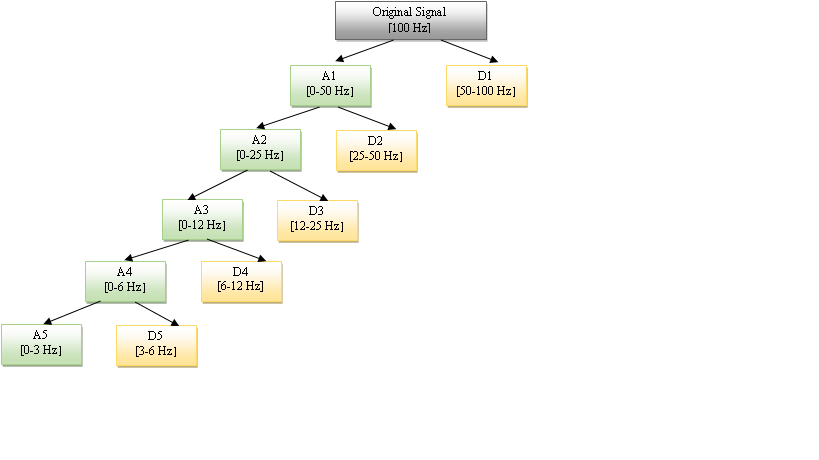
\includegraphics[width=1\textwidth]{DWT.png}

\caption{Sub-band decomposition of DWT implementation}
\end{figure}
%------------------------------------------------
\begin{figure}

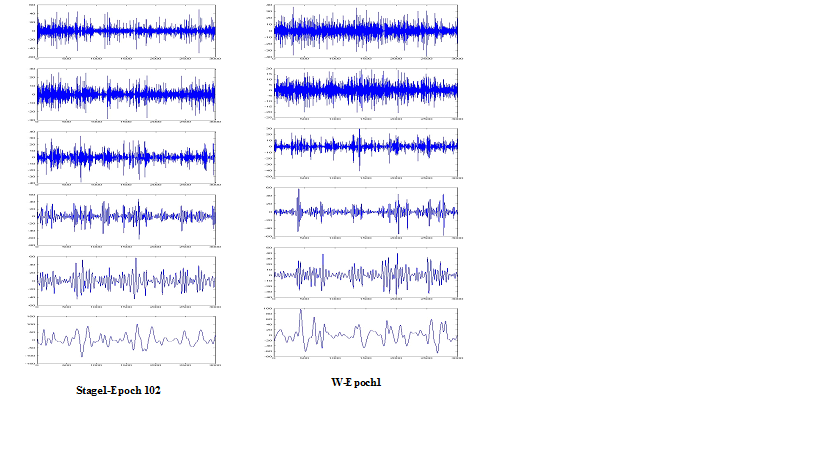
\includegraphics[width=1\textwidth]{stages.png}

\caption{Sleep Decomposition}
\end{figure}
\section*{Specifications of Dataset}

The EEG dataset is available online at PhysioBank [8]. The polysmnographic (PSG) sleep recordings included signals from EEG ( Fpz-Cz and Pz-Oz channels), horizontal EOG, submental chin EMG and an event marker. Well-trained technicians scored manually hypnograms based on the 1968 Rechtschaffen and Kales manual [9].
There are two subsets of data. In the first set, 20 healthy subjects were selected in order to study the effects of age on sleep. Two EEG datasets (about 20 hours) were recorded during two subsequent day-night periods for each subject at their home. In the second dataset, 22 subjects that had difficulty in falling sleep were selected from a study of Temazepam effects on sleep. The PSGs (about 9 hours) were recorded in the hospital during two nights.




\section*{Literature Review}\label{sec:lit_review}
\looseness - 1
\section*{Acknowledgments}
The authors were partially supported by 

%We also thank the Associate Editor and the anonymous referee for their insightful and constructive comments.



\bibliographystyle{plain}
*\bibliographystyle{unsrt}
*\bibliography{}


%\newpage
%\section{Appendix}\label{app:1}





\end{document}
